
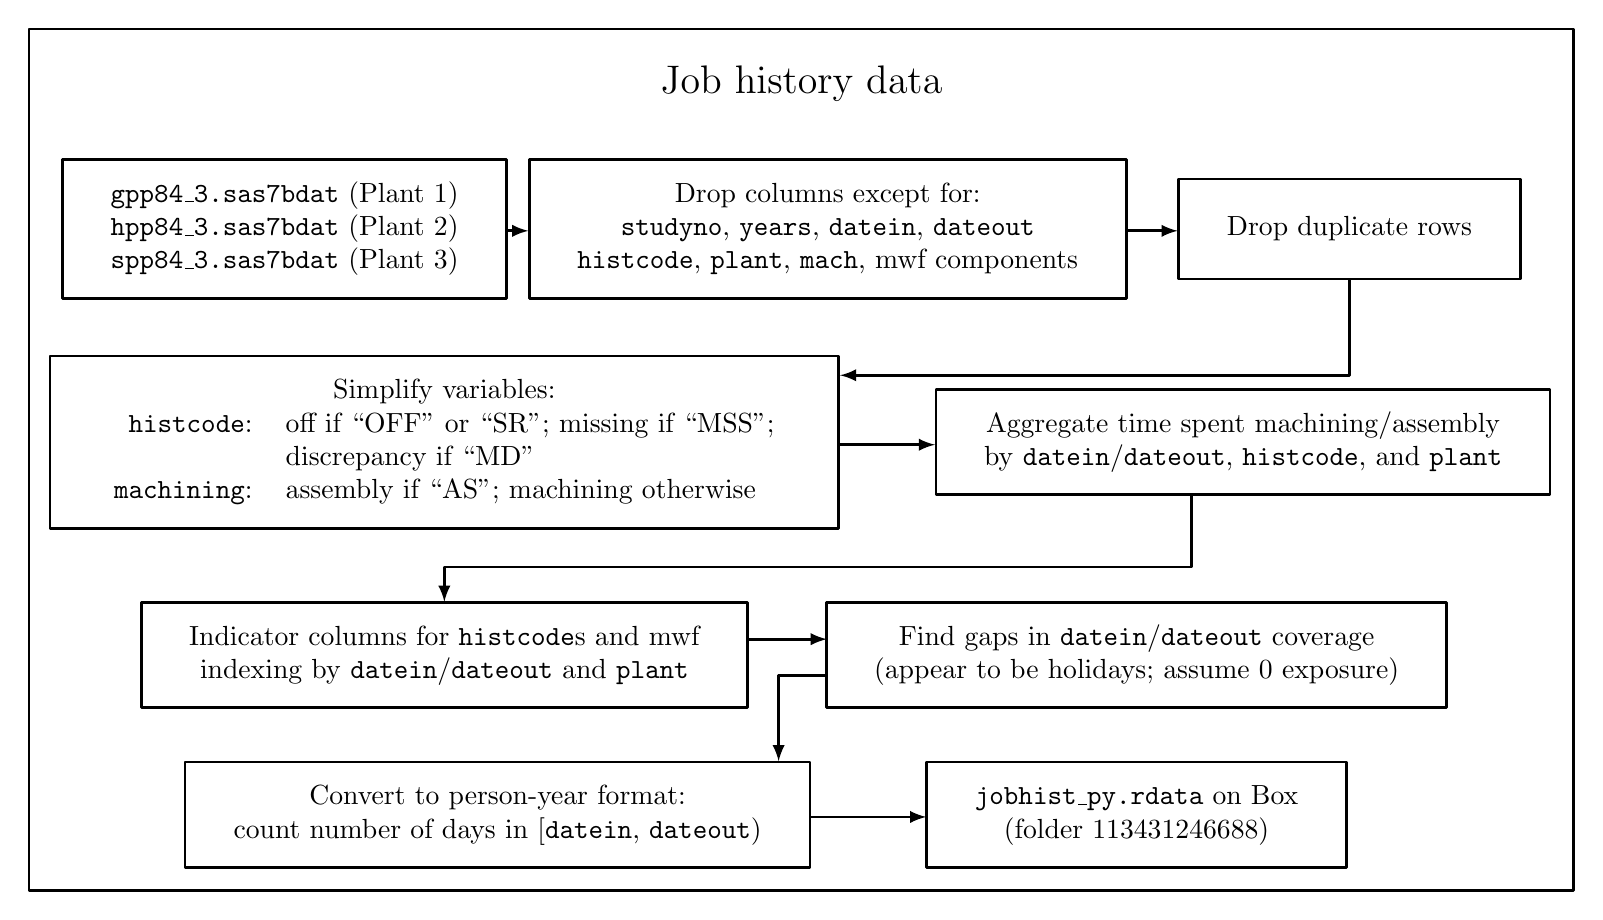
\begin{tikzpicture}[>=latex,line join=bevel,]
  \pgfsetlinewidth{1bp}
%%
\begin{scope}
  \pgfsetstrokecolor{black}
  \definecolor{strokecol}{rgb}{0.0,0.0,0.0}
  \pgfsetstrokecolor{strokecol}
  \draw (0.24bp,-0.36bp) -- (0.24bp,309.64bp) -- (556.24bp,309.64bp) -- (556.24bp,-0.36bp) -- cycle;
  \draw (278.24bp,290.14bp) node {\Large Job history data};
\end{scope}
  \pgfsetcolor{black}
  % Edge: filter -> drop
  \draw [->] (395.4bp,237.0bp) .. controls (395.4bp,237.0bp) and (403.73bp,237.0bp)  .. (413.73bp,237.0bp);
  % Edge: drop -> simplify
  \draw [->] (475.61bp,219.52bp) .. controls (475.61bp,204.3bp) and (475.61bp,185.0bp)  .. (475.61bp,185.0bp) .. controls (475.61bp,185.0bp) and (302.2bp,185.0bp)  .. (292.2bp,185.0bp);
  % Edge: machining -> histcode
  \draw [->] (418.6bp,141.9bp) .. controls (418.6bp,129.64bp) and (418.6bp,116.0bp)  .. (418.6bp,116.0bp) .. controls (418.6bp,116.0bp) and (149.74bp,116.0bp)  .. (149.74bp,116.0bp) .. controls (149.74bp,116.0bp) and (149.74bp,113.47bp)  .. (149.74bp,103.47bp);
  % Edge: job -> filter
  \draw [->] (172.33bp,237.0bp) .. controls (172.33bp,237.0bp) and (173.09bp,237.0bp)  .. (179.96bp,237.0bp);
  % Edge: simplify -> machining
  \draw [->] (291.82bp,160.0bp) .. controls (291.82bp,160.0bp) and (316.37bp,160.0bp)  .. (326.37bp,160.0bp);
  % Edge: histcode -> cont
  \draw [->] (259.04bp,90.0bp) .. controls (259.04bp,90.0bp) and (277.42bp,90.0bp)  .. (287.42bp,90.0bp);
  % Edge: cont -> clean
  \draw [->] (287.19bp,77.0bp) .. controls (276.81bp,77.0bp) and (270.08bp,77.0bp)  .. (270.08bp,77.0bp) .. controls (270.08bp,77.0bp) and (270.08bp,56.057bp)  .. (270.08bp,46.057bp);
  % Edge: clean -> final
  \draw [->] (281.57bp,26.0bp) .. controls (281.57bp,26.0bp) and (313.2bp,26.0bp)  .. (323.2bp,26.0bp);
  % Node: cont
\begin{scope}
  \definecolor{strokecol}{rgb}{0.0,0.0,0.0}
  \pgfsetstrokecolor{strokecol}
  \draw (510.44bp,103.29bp) -- (287.44bp,103.29bp) -- (287.44bp,65.29bp) -- (510.44bp,65.29bp) -- cycle;
  \draw (398.94bp,84.292bp) node {\begin{tabular}{c} 
						Find gaps in \texttt{datein}/\texttt{dateout} coverage \\						(appear to be holidays; assume 0 exposure)
						\end{tabular}};
\end{scope}
  % Node: drop
\begin{scope}
  \definecolor{strokecol}{rgb}{0.0,0.0,0.0}
  \pgfsetstrokecolor{strokecol}
  \draw (537.11bp,255.64bp) -- (414.11bp,255.64bp) -- (414.11bp,219.64bp) -- (537.11bp,219.64bp) -- cycle;
  \draw (475.61bp,237.64bp) node {\begin{tabular}{c} 
						Drop duplicate rows
						\end{tabular}};
\end{scope}
  % Node: filter
\begin{scope}
  \definecolor{strokecol}{rgb}{0.0,0.0,0.0}
  \pgfsetstrokecolor{strokecol}
  \draw (395.26bp,262.64bp) -- (180.26bp,262.64bp) -- (180.26bp,212.64bp) -- (395.26bp,212.64bp) -- cycle;
  \draw (287.76bp,237.64bp) node {\begin{tabular}{c} 
						Drop columns except for: \\						\texttt{studyno}, \texttt{years}, \texttt{datein}, \texttt{dateout} \\						\texttt{histcode}, \texttt{plant}, \texttt{mach}, mwf components \\						\end{tabular}};
\end{scope}
  % Node: simplify
\begin{scope}
  \definecolor{strokecol}{rgb}{0.0,0.0,0.0}
  \pgfsetstrokecolor{strokecol}
  \draw (291.74bp,191.97bp) -- (7.74bp,191.97bp) -- (7.74bp,129.97bp) -- (291.74bp,129.97bp) -- cycle;
  \draw (149.74bp,160.97bp) node {\begin{tabular}{c} 
						Simplify variables: \\								\begin{tabular}{rl}
								\texttt{histcode}: & off if ``OFF'' or ``SR'';
								missing if ``MSS''; \\								& discrepancy if ``MD'' \\								\texttt{machining}: & assembly if ``AS''; machining otherwise
								\end{tabular}
						\end{tabular}};
\end{scope}
  % Node: job
\begin{scope}
  \definecolor{strokecol}{rgb}{0.0,0.0,0.0}
  \pgfsetstrokecolor{strokecol}
  \draw (172.24bp,262.64bp) -- (12.24bp,262.64bp) -- (12.24bp,212.64bp) -- (172.24bp,212.64bp) -- cycle;
  \draw (92.238bp,237.64bp) node {\begin{tabular}{c} 
						\texttt{gpp84\_3.sas7bdat} (Plant 1) \\						\texttt{hpp84\_3.sas7bdat} (Plant 2) \\						\texttt{spp84\_3.sas7bdat} (Plant 3) \\						\end{tabular}};
\end{scope}
  % Node: machining
\begin{scope}
  \definecolor{strokecol}{rgb}{0.0,0.0,0.0}
  \pgfsetstrokecolor{strokecol}
  \draw (547.77bp,179.97bp) -- (326.77bp,179.97bp) -- (326.77bp,141.97bp) -- (547.77bp,141.97bp) -- cycle;
  \draw (437.27bp,160.97bp) node {\begin{tabular}{c} 
						Aggregate time spent machining/assembly \\						by \texttt{datein}/\texttt{dateout}, \texttt{histcode}, and \texttt{plant}
						\end{tabular}};
\end{scope}
  % Node: clean
\begin{scope}
  \definecolor{strokecol}{rgb}{0.0,0.0,0.0}
  \pgfsetstrokecolor{strokecol}
  \draw (281.41bp,45.79bp) -- (56.41bp,45.79bp) -- (56.41bp,7.79bp) -- (281.41bp,7.79bp) -- cycle;
  \draw (168.91bp,26.786bp) node {\begin{tabular}{c} 
						Convert to person-year format: \\						count number of days in [\texttt{datein}, \texttt{dateout})
						\end{tabular}};
\end{scope}
  % Node: histcode
\begin{scope}
  \definecolor{strokecol}{rgb}{0.0,0.0,0.0}
  \pgfsetstrokecolor{strokecol}
  \draw (258.74bp,103.29bp) -- (40.74bp,103.29bp) -- (40.74bp,65.29bp) -- (258.74bp,65.29bp) -- cycle;
  \draw (149.74bp,84.292bp) node {\begin{tabular}{c} 
						Indicator columns for \texttt{histcode}s and mwf\\						indexing by \texttt{datein}/\texttt{dateout} and \texttt{plant}
						\end{tabular}};
\end{scope}
  % Node: final
\begin{scope}
  \definecolor{strokecol}{rgb}{0.0,0.0,0.0}
  \pgfsetstrokecolor{strokecol}
  \draw (474.44bp,45.79bp) -- (323.44bp,45.79bp) -- (323.44bp,7.79bp) -- (474.44bp,7.79bp) -- cycle;
  \draw (398.94bp,26.786bp) node {\begin{tabular}{c} 
						\texttt{jobhist\_py.rdata} on Box \\						({folder 113431246688})
						\end{tabular}};
\end{scope}
%
\end{tikzpicture}

